\documentclass[12pt]{article}

\usepackage{graphicx}
\graphicspath{ {imgs/} }

\usepackage[utf8]{inputenc}

\usepackage{listings}
\usepackage{color}

\lstdefinestyle{mystyle}{
    backgroundcolor=\color{backcolour},
    commentstyle=\color{codegreen},
    keywordstyle=\color{magenta},
    numberstyle=\tiny\color{codegray},
    stringstyle=\color{codepurple},
    basicstyle=\footnotesize,
    breakatwhitespace=false,
    breaklines=true,
    captionpos=b,
    keepspaces=true,
    numbers=left,
    numbersep=5pt,
    showspaces=false,
    showstringspaces=false,
    showtabs=false,
    tabsize=2
}
\lstset{
  frame=none,
  xleftmargin=2pt,
  stepnumber=1,
  numbers=left,
  numbersep=5pt,
  numberstyle=\ttfamily\tiny\color[gray]{0.3},
  belowcaptionskip=\bigskipamount,
  captionpos=b,
  escapeinside={*'}{'*},
  language=haskell,
  tabsize=2,
  emphstyle={\bf},
  commentstyle=\it,
  stringstyle=\mdseries\rmfamily,
  showspaces=false,
  keywordstyle=\bfseries\rmfamily,
  columns=flexible,
  basicstyle=\small\sffamily,
  showstringspaces=false,
  morecomment=[l]\%,
}

\usepackage{upgreek}

\usepackage{amsmath}

\usepackage{graphicx}
\graphicspath{ {imgs/} }

\usepackage{enumitem}

\usepackage{listings}

\usepackage{mathtools}
\DeclarePairedDelimiter\ceil{\lceil}{\rceil}
\DeclarePairedDelimiter\floor{\lfloor}{\rfloor}

\usepackage{color}

\definecolor{codegreen}{rgb}{0,0.6,0}
\definecolor{codegray}{rgb}{0.5,0.5,0.5}
\definecolor{codepurple}{rgb}{0.58,0,0.82}
\definecolor{backcolour}{rgb}{0.95,0.95,0.92}

\lstdefinestyle{mystyle}{
    backgroundcolor=\color{backcolour},
    commentstyle=\color{codegreen},
    keywordstyle=\color{magenta},
    numberstyle=\tiny\color{codegray},
    stringstyle=\color{codepurple},
    basicstyle=\footnotesize,
    breakatwhitespace=false,
    breaklines=true,
    captionpos=b,
    keepspaces=true,
    numbers=left,
    numbersep=5pt,
    showspaces=false,
    showstringspaces=false,
    showtabs=false,
    tabsize=2
}

\lstset{style=mystyle}

\usepackage{dsfont}

\usepackage{hyperref}

\usepackage[utf8]{inputenc}

\usepackage{mathtools}

\usepackage{textcomp}

\usepackage[english]{babel}

\usepackage{tikz}

\usepackage{tcolorbox}

\usepackage{amsthm,amssymb}

\setlength{\parindent}{0cm}

\renewcommand\qedsymbol{$\blacksquare$}

\usepackage{fancyhdr}

\pagestyle{fancy}
\fancyhf{}
\fancyhead[LE,RO]{Principles of Programming Languages -- Winter 2018}
\fancyhead[RE,LO]{Joshua Concon}
\fancyfoot[CE,CO]{\leftmark}
\fancyfoot[LE,RO]{\thepage}


\begin{document}

\title{CSCC24: Principles of Programming Languages\\ Notes}
\date{University of Toronto Scarborough -- Winter 2018}
\author{Joshua Concon}
\maketitle
This course is taught by Dr. Albert Yu Cheong Lai. If you find any problems in these notes, feel free to contact me at conconjoshua@gmail.com.

\tableofcontents

\pagebreak

\section{Thursday, January 11, 2017}

The purpose of this course is to see the trade-offs between various features in programming languages. This course exists because different programming languages have different features, for example, Java has both class-based OOP and auto-garbage collection while C has neither, but C has union types that Java doesn't have. This means rewriting code into a different language isn't necessarily easy. There may be large semantic differences

\subsection{The Root Cause of this Course}

A guy named "John Backus" gave a lecture for the acceptance for the Turing Award in 1977. He addressed the question, "Can programming be liberated from the von Neumann style?"\\
\\
Languages then had been only superficial enhancements to the CPU writing 1 word onto memory at a time i.e:

\begin{lstlisting}
	s := s + a[i]
\end{lstlisting}

Backus proposed a new direction for programming languages:
\begin{itemize}
    \item Higher order functions that work on aggregates (a whole list, an array, a dictionary, etc...)
    \item Combining forms, for example, function composition ($g \circ f$)
    \item Reasoning by algebra, for example, the associative law for a function
    \item If you need a state, use coarse-grained state transitions rather than changing only one word at a time. (So passing an old state into a stateless function that does a lot and returns an answer and a new state.)
\end{itemize}

\subsubsection{Higher-order Functions on Aggregates}

Note that the notation to apply a function to several parameters is:
\\(Haskell)
\begin{lstlisting}[language=Haskell]
    f x y z
\end{lstlisting}
(Scheme:)
\begin{lstlisting}
    (f x y z)
\end{lstlisting}

So in Haskell:
\begin{lstlisting}[language=Haskell]
    fmap f [x0, x1, ...]
\end{lstlisting}

will compute

\begin{lstlisting}[language=Haskell]
    [f x0, f x1, ...]
\end{lstlisting}

And

\begin{lstlisting}[language=Haskell]
    fmap abs [3,-1,4]
\end{lstlisting}

Computes

\begin{lstlisting}[language=Haskell]
    [3,-1,4]
\end{lstlisting}

And

\begin{lstlisting}[language=Haskell]
    folder (+) 0 [3,1,4]
\end{lstlisting}

Computes

\begin{lstlisting}[language=Haskell]
    3+(1+(4+0))
\end{lstlisting}

Note 2 points:
\begin{itemize}
    \item "on aggregates" means to work on a whole list at once (such as an array or some "container")
    \item "Higher-order functions" means that some parameters are functions, so different combinations makes the language more customizable.
\end{itemize}

Java and MATLAB have the former but lack the latter.

\subsubsection{Combining Forms}

An obvious example is function composition $(g \circ f)$.

In Haskell, this is:
\begin{lstlisting}[language=Haskell]
    g . f
\end{lstlisting}

And in Racket (Scheme) this is:
\begin{lstlisting}
    compose g f
\end{lstlisting}

For example, the following code computes the 1-norm of your vector.

\begin{lstlisting}[language=Haskell]
    foldr (+) 0 . fmap abs
\end{lstlisting}

There are other combining forms. There is another example in Haskell.

\begin{lstlisting}[language=Haskell]
    (f &&& g) x = (f x, g x)
\end{lstlisting}

The point is that you can combine functions to perform compound tasks, and this type of language is not about shorter code (although it has that side effect), but about working with building blocks.

\subsubsection{Example Topic: Evaluation Order}

You can define your own logical "and" in Scheme

\begin{lstlisting}
    (define (my-and b c) (if b c #f))
    (my-and #f (list-ref '(#t #f #t) 10))
\end{lstlisting}

The second line fails in Scheme, but if typed in the Haskell version, succeeds.\\
\\
In most languages, parameters are evaluated before passed into the bodies of functions. In Haskell however, parameters are passed as is. Because of this, in Haskell, many short circuiting operators and control constructs are user-definable, and therefore, very customizable.

\subsubsection{Example Topic: Scheme Macros}

Scheme offers a macro system for user-defined constructs:

\begin{lstlisting}
    (define-syntax-rule (my-and b c) (if b c #f))
\end{lstlisting}

Now if we run the following code, it succeeds.

\begin{lstlisting}
    (my-and #f (list-ref '(#t #f #t) 10))
\end{lstlisting}

The explanation for this is that this is a macro expansion in Scheme, so the parameters are copy-pasted into the macros. This means that there is a downside, for example:

\begin{lstlisting}
    (define-syntax-rule (double x) (+ x x))
    (double (* 3 4))
\end{lstlisting}

The second line spawns two copies of (* 3 4) and performs redundant work, while Haskell's version does not. The Upside is that Scheme's macro system offers other flexibilities not shown in this lecture.

\subsubsection{Dynamic and Static Typing}

In Scheme:
\begin{lstlisting}
    (if #f 0 (+ 0 "hello"))
    (if #t 0 (+ 0 "hello"))
\end{lstlisting}

The first line fails but the second line succeeds. This is because Types are checked dynamically. When running the program, only the code that is actually run is checked.

In Haskell, the following line fails:
\begin{lstlisting}
    if True then 0 else 0 + "hello"
\end{lstlisting}

The reason for this is because types are checked statically, without running, over all the code. (If this code is compiled, then at compile time, if interpreted, then at load time, etc.) So the error of adding 0 to "hello".\\
\\
Food for though, Java is both compiled and interpreted.

\subsubsection{Parametric Polymorphism}

In Haskell, we define:

\begin{lstlisting}
    trio x = [x, x, x]
\end{lstlisting}
The inferred type is:
\begin{lstlisting}
    a -> [a]
\end{lstlisting}
This is analogous to Java's
\begin{lstlisting}
    <T> LinkedList<T> trio(<T> x)
\end{lstlisting}

\underline{Note:} That the following 2 lines are both legal if we have trio defined
\begin{lstlisting}
    trio 0
    trio "hello"
\end{lstlisting}

"Parametric" means:
Supposed you have defined $d$ of type $a \mapsto [a]$, Then you would need one test to know what it does. Say we test $d True$ and the answer has length 2. Then we can deduce that $d x$ returns $[x,x]$ for all $x$.\\
\\
The basic explanation for this is that $d$ cannot vary behaviour by types. Haskell allows type-determined behaviour, but the function type will look like:
\begin{lstlisting}
    Foo a => a -> [a]
\end{lstlisting}

\subsubsection{What is "Powerful"? -- The Tradeoff}

"Macro systems, dynamic typing, ... are powerful." This refers to the flexibility for the implementer or the original author.\\
\\
"Static typing, parametric polymorphism... are powerful." This refers to the predictability for the user or the maintainer.\\
\\
Programming is a dialectic class struggle between the user and the implementer. Or between the maintainer and the original author.

\newpage

\section{Thursday, January 18, 2018}

\subsection{Racket}

We won't be using just Scheme, we'll be using Racket which is a version of Scheme. Racket is a platform for implementing and using many languages, and Scheme is on of those that come out of the box.\\
\\
Racket's version of scheme is somewhat different from the standards with regards to function names, and some features. We will cover Racket, but note that these examples and features may fail for standard Scheme.

\subsection{Basic Data Types}

\begin{lstlisting}
    #t, #f ;booleans
    42 ;numbers, can be ints, rational, floats, complex
    "hello" ; strings
    #\h ; this is a char of just the letter h
    'Chrome ;this is a symbol
\end{lstlisting}

\paragraph{Symbols} Symbols are user-defined atomic values. You think of a name, put a single quote in front. Symbols are not strings, you can't perform string operations onto them.

\subsection{Procedures and Functions}
For example:
\begin{lstlisting}
    (sin (/ 0.2 2)) ; sine of 1 over 10
\end{lstlisting}

\subsection{Boolean Operations}

\begin{lstlisting}
    (not expr)
    (and expr expr)
    (or expr expr)
    (or) ; gives #f
    (and) ; gives #t
    (boolean? expr) ; tests if you have a boolean
\end{lstlisting}

\subsection{Number operations}

\begin{lstlisting}
    +
    -
    *
    /
    max
    min
    -
    <
    >
    <=
    >=
    ; these operations can all take multiple operands
\end{lstlisting}

\begin{lstlisting}
    number?
    complex?
    real?
    rational?
    ; these functions test if a number is a certain type
\end{lstlisting}

\subsection{Equality}

There are 3 types of equalities.

\begin{lstlisting}
    eq?
\end{lstlisting}
	This one is Good for booleans and symbols, uses pointer inequality for aggregates like strings and lists, but has complicated rules for numbers.

\begin{lstlisting}
    eqv?
\end{lstlisting}
	This one has complicated rules for numbers as well, and different from eq? as it treats the floating-points NaN and signed zero differently.

	\begin{lstlisting}
    equal?
\end{lstlisting}
This one is for structural equality for most aggregates. So comparing contents of an aggregate.

\subsection{Definitions}

You can define functions and constants, recursion is allowed.

\begin{lstlisting}
; A constant
(define my-width/height (/ 4 3))
; a function with 2 parameters
(define (my-log base x)
	(/ (log x) (log base)))

\end{lstlisting}

\subsection{Anonymous Functions}

Basically a function without a name, you can either right lambda or use $\lambda$ in your code.\\
\\
Example of a function:
\begin{lstlisting}
    (lambda (base x) (/ (log x) (log base)))
\end{lstlisting}
Example of the same function being used
\begin{lstlisting}
    ((lambda (base x) (/ (log x) (log base))) 128 2)
\end{lstlisting}
So in this case, base passed in as 128 and x as 2

\subsection{Conditionals}

If-then-else conditions look like the following
\begin{lstlisting}
	(if test then-expr else-expr)
\end{lstlisting}
Test can be non-boolean, and this will be treated as true.

Multiple conditions are as such:
\begin{lstlisting}
	(cond
		[(> x y) (sin x)]
		[(< x y) (cos y)]
		[else 0])
\end{lstlisting}
This is if $x>y$ then $sinx$ else if $x < y$ then $cosy$ else 0. Test results can be non-boolean, which are treated as true. You can obtain the result of a test to return it.
\begin{lstlisting}
	(cond
		[(+ 4 2) => (lambda (x) (* x x))]
		[else 0])
\end{lstlisting}
This gives 36.

\subsubsection{and,or as conditionals}
\textbf{and} evaluates all of its operands from left to right and stops as soon as \#f operand is read, otherwise the last expression is the answer.\\
\\
\textbf{or} evaluates all of its operands from left to right and stops as soon as a non \#f operand is read, and that becomes the answer, otherwise the answer is \# f

\subsection{Local bindings}

Local definitions for use in just one expression

\begin{lstlisting}
	(let ([x expr1]
		[y expr2])
		(+ x y (* 2 x y)))
\end{lstlisting}
This means to compute $x+y+2xy$ where $x=expr1$ and $y=expr2$. These 2 expressions cannot see the others variables, only the global ones outside of their scope.
\begin{lstlisting}
	(let ([x 3])
		(let ([x (* 3 3)]) ; (* 3 3)
		x))
\end{lstlisting}
This results in 9 and is not recursive. Let* allows later bindings to see earlier bindings
\begin{lstlisting}
	(let* ([x 5]
		[y (+ x 1)]) ; (+ 5 1)
		(+ x y (* 2 x y)))
\end{lstlisting}
\subsubsection{Recursive local bindings}

letrec allows more recursive bindings

\begin{lstlisting}
	(letrec ([fac
		(lambda (n)
			(if (= n 0) 1 (* n (fac (- n 1)))))]
		[even
			(lambda (n)
				(or (= n 0) (not (odd (- n 1)))))]
		[odd
			(lambda (n)
				(not (even (- n 1))))])
	(even (fac 5)))
\end{lstlisting}
This returns whether or not factorial 5 is even. So true.

\subsection{Recommended Code Layout}

\begin{itemize}
	\item{Open parentheses then immediately first word}
	\item{Procedure definition: Body starts on new line, indented}
	\item{Long expression: Parts start on new lines, indented}
	\item{Closing parentheses not on new lines}
\end{itemize}

\newpage

\section{Thursday, January 25, 2018}

\subsection{Pairs and Lists}

A cons cell is a 2-tuple pair and has the following syntax:
\begin{lstlisting}
	cons(x y)
\end{lstlisting}
Essentially a pair of pointers. Has special support for lists.
\begin{lstlisting}
	'() ; an empty list
	(list x y z) = (cons x (cons y (cons z '())))
	'(42 "hi" Chrome)
	; Chrome here will be the symbol 'Chrome
\end{lstlisting}

For a cons cell, you can use car to access the first field and cdr to access the second field.

\subsection{User-Defined Records}

\begin{lstlisting}
	(struct dim (width height))
\end{lstlisting}
This creates a new record type with 2 fields
\begin{lstlisting}
	(dim 4 7) ; this constructs a vlue of this type
	dim? ; this tests for this type
	dim-width
	dim-height
	; these are the field accessors
\end{lstlisting}

We can also use struct-copy to clone a record while replacing some values:
\begin{lstlisting}
	(define d1 (dim 4 7))
	(define d2 (struct-copy dim d1 [width 5]))
	; d2 is (dim 5 7)
\end{lstlisting}

\subsection{Pattern Matching}

You can test for a literal, cons cell, or a record type, can get their content as well.

\begin{lstlisting}
	(struct dim (width height))

	(define (foo x)
		(match x
			['() 'nada]
			[(cons b _) b]
			[(dim w h) (* w h)]))
	(foo '()) ; returns 'nada
	(foo '(1 2 3)) ; returns 1
	(foo (dim 4 7)) ; returns 28
\end{lstlisting}

\subsection{Input and Output}

We can print with display, printf and displayln

\begin{lstlisting}
	(display 5)
	(newline)
	(displayln 5)
	(printf "yes" "price" 5)
\end{lstlisting}

\begin{lstlisting}
	(read-line) ; this reads a lien
	(read-string 10) ; this reads up to the upper bound.
	;if it reaches the end of the file, it returns eof, which you can use eq? or eof-object? to test
	; for stderr, eprintf is like printf but goes to stderr
\end{lstlisting}

\subsubsection{ports}

Racket has ports, analogous to Java Reader/Writer -- behind it can be file, string, network connection, message queue, user-defined, etc.

\subsection{Sequencing}

If we want to evaluate multiple expressions in the order we specify

\begin{lstlisting}
	(begin
		(display ln "Please enter your name")
		(read-line)) ; this returns the last expression

	(begin0 expr1 expr2) ; this returns the first expression, but the others are still evaluated.

	(when (> x 0) expr1 expr2 ...)
	; if true, evaluates the exoressions, returns what the last one returns, if false, returns #<void>
\end{lstlisting}

\subsection{Mutable Varibles}

\begin{lstlisting}
	(define v 5)
	(define (f x) (+ x v))
	(f 0) ; this gives 5
	(set! v 6)
	(f 0) ; this gives 6
\end{lstlisting}

Mutable paris, list, strings, arrays, etc. are also available. Use mutation judiciously, is not that necessary.

\subsection{map}

Takes in a function and a list and applies the function to every element in that list

\begin{lstlisting}
	(map f (list x y z)) = (list (f x) (f y) (f z))
\end{lstlisting}

\subsection{filter}

filter takes in a boolean function and a list (A) and returns a list of the items in the list A that satisfy the boolean function

\begin{lstlisting}
	(filter number? '(9 "4" 0 "1" "6" 5)) = '(9 0 5)
\end{lstlisting}


\newpage

\section{Thursday, February 1, 2018}

\subsection{Scheme (cont'd)}

\subsubsection{foldl}

Consider the problem of summing an entire list and multiplying an entire list. Summing requires us to add up all the elements of the list plus 0 for the first item. Multiplying requires us to multiply up all the elements of the list times 1 for the first item. This is the motivation.\\
\\
So we define foldl as

\begin{lstlisting}
    (define (foldl binop a lst)
	(match lst
	[?() a]
	[( cons hd tl) (foldl binop (binop a hd) tl )]))
\end{lstlisting}

So Intuitively,

\begin{lstlisting}
	(foldl binop a (list x y z))
\end{lstlisting}

Looks like

$$(((a + x) + y) + z)$$

where $+$ is where binop is being performed

\subsubsection{foldr}

Basically in the opposite direction of foldl, so if

\begin{lstlisting}
	(foldl binop a (list x y z))
\end{lstlisting}

Looks like

$$(z + (y + (x+a)))$$

where $+$ is where binop is being performed, then

\begin{lstlisting}
	(foldr binop a (list x y z))
\end{lstlisting}

Looks like

$$(((a + x) + y) + z)$$

where $+$ is where binop is being performed, then

\subsubsection{Procedure-Call Stack}

Consider the following:

\begin{lstlisting}
	(define (f n) (... (f (- n 1)) ...)
	(displayln (+ (f 4) (f 1) (f 6)))
\end{lstlisting}

The Control-flow jumps to into $f$ when it's called and later knows where to return to after the recursive calls. This is done because a stack is used to remember where to return to in recursion, called a \textbf{Call Stack}. The Benefit of this is that it supports recursion, but it comes at a price of occupying $\theta (1)$ space while the stack is being used.

\subsubsection{Non-Tail Calls and Tail Calls}

\textbf{Non-Tail Calls}, are if you still have to do your own processing or computation after getting the results from another function, so basically the results are not returned right away.
\\
\\
For example, for the following function:

\begin{lstlisting}
	(define (my -sum lst)
		(match lst [?() 0]
				[( cons hd tl) (+ hd (my -sum tl ))]))
\end{lstlisting}

Takes $\theta (n)$ space if the list length is $n$.\\
\\
A Tail call is the exact opposite, there is no computation after getting the results back from a called function and the function returns the value right away. The complexity of this is $O(1)$ under Tail-Calling optimization in Scheme.\\
\\
Tail-Calling optimization isn't in every language, Java and Python don't have this.

\subsection{Haskell}

\subsubsection{Expressions and Types}

\paragraph{Characters} chars are denoted with single quotes

\paragraph{Tuples} Not the same as cons

\paragraph{()} is a special time, called the unit type, used as a return value for functions that don't return anything

\paragraph{Lists} Lists are implemented as such:

\begin{lstlisting}
	3 : ( 1 : (4 : [])) = [3,1,4]
\end{lstlisting}

So a list of length one is an item with an empty list and the colon inbetween separates the items
\begin{lstlisting}
	[1] = 1 : []
\end{lstlisting}

Note that the following list has a type $[[integer]]$

\begin{lstlisting}
	[[3,1,4], [10,20], []]
\end{lstlisting}

So as for now, arbitrary list nesting is not supported, so basically

\begin{lstlisting}
	[1, [3]]
\end{lstlisting}

is not supported (yet).

Note that because of static typing, every item must be the same type, we can't mix integers with floats in the same list.

\paragraph{Strings} are a list of chars. The downside of this is that it uses a huge amount of memory, as it's stored as a linked list, and each node and pointer takes up a linear amount of space.

\paragraph{Keyword: Just} If you type

\begin{lstlisting}
	Just 'C'
\end{lstlisting}

The variable is either Nothing or Char

\paragraph{Nothing} Is the empty type, can be any type

\paragraph{"Left 'C'"} Can either be of type Char Bool, Char Int,  ... all we know that the left variable is a character.

\paragraph{"Right False"} Can either be of type Char bool, Int bool, ... all we know that the right variable is a boolean

\paragraph{anonymous functions} Ex.

\begin{lstlisting}
	 \x -> x >= 'C'
\end{lstlisting}

Has the type Char -$>$ Bool with char as the domain and bool as the codomain

\subsubsection{Definitions}

We can define expressions to variables and vice versa, for example, in the following, we are defining "ten" to be "$1+2+3+4$" and binding "$1+2+3+4$" to "ten":
\begin{lstlisting}
	ten = 1 + 2 + 3 + 4
\end{lstlisting}

There is also pattern binding, with tuples, but that will be shown later\\
\\
Functions can also be defined:

\begin{lstlisting}
	square x = x * x
	nand a b =  not (a && b)
\end{lstlisting}

We can also define type signatures for the definitions as such

\begin{lstlisting}
	ten, four :: Integer
\end{lstlisting}

But Haskell is written such that the type signature can be separated from the definition, so you don't have to put them in the same few lines, they just have to be in the same file.

\subsubsection{Function Applications}

If you insert one parameter to a function that takes 2 parameters, that function will return a function of 1 parameter. This is how Haskell does multiple parameters

\newpage

\section{Thursday, February 8, 2018}

\subsection{Haskell (cont'd)}

\subsubsection{Local Definitions For Expressions}

\begin{lstlisting}
	let x = 4 + 5
	     y = 4 - 5
	 in x+y+2*x*y
\end{lstlisting}

Layout Version above. Braced Version below

\subsubsection{Local Definitions For Definitions}

\begin{lstlisting}
	foo u v = x + y + 2*x*y
		where -- this where refers to the statement in line 1
			x = u + v
			y= u - v
\end{lstlisting}

\subsubsection{Pattern Matching}

Can be done for expressions or function definitions as well as pattern binding.

\begin{lstlisting}
-- expression case
case expr of
	[] -> 0
	42 : xs -> foo xs
	x : xs -> x + foo xs
\end{lstlisting}

In this example, the expression $expr$ would evaluate to 0 if it was an empty list, have foo applied to its tail if it started with 42 as its first index and x plus foo applied to its tail for any other list.

\begin{lstlisting}
-- function definition case examples

mySum [] = 0
mySum (x : xs) = x + mySum xs

nand False _ = True
nand True False = True
nand True True = False
\end{lstlisting}

\begin{lstlisting}
-- pattern binding case
[a, b, c] = take 3 someList
-- a = take
-- b = 3
-- c = someList
\end{lstlisting}

\subsubsection{Guards}

Guards are extra conditions imposed on patterns.

\begin{lstlisting}
-- expression case
case expr of
	[] -> 0
	x : xs | x < 0 -> x + foo xs
		  | x > 2 -> x - foo xs
		  | True -> x * foo xs

-- definition case
foo [] = 0
foo (x : xs) | x < 0 -> x + foo xs
		  | x > 2 -> x - foo xs
		  | True -> x * foo xs
\end{lstlisting}

Instead of True for the edge case, can also use "otherwise".

\subsubsection{Local Definitions under Patterns and Guards}

\begin{lstlisting}
foo :: Either String Integer -> Integer
foo (Left str) | suffix > "albert" = 42
		    | otherwise = 24
		    where
		    	suffix = drop 10 str

foo (Right x) | x > 0 = 2*y
		     | x < 0 = y
		     | otherwise = 0
		     where
		     	y = div 1000 x
\end{lstlisting}
Note that the first where belongs to the foo where the input is a Left str, the second where belongs to the foo where the input is a Right integer and if $x=0$, then $y$ will not be calculated.

\subsubsection{List Comprehension}

\begin{lstlisting}
	[x + y | x <- [10,20,30], x > 10, y <- [4,5] ]
	-- this results in
	--[20+4, 20+5, 30+4, 30+5]
\end{lstlisting}

We can use pattern matching as well

\begin{lstlisting}
	[x+3 | Just x <= [Just 10, Nothing, Just 30]]
	-- this results in
	-- [10+3, 30+3]
\end{lstlisting}

There is also a range notation we can use:

\begin{lstlisting}
	[1...5] -- this is the same as [1,2,3,4,5]
\end{lstlisting}

\subsubsection{Algebraic Data Types}

\begin{lstlisting}
	data MyType = Nada | Duplet Double String | Uno Integer
\end{lstlisting}

Nada, Duplet, Uno are data constructors. They must start with uppercase letters. They form expressions and patterns.\\
\\
The following is an example function that takes in "MyType":

\begin{lstlisting}
plus1 :: MyType -> MyType
plus1 Nada = Nada
plus1 (Duplet r s) = Duplet (r+1) s
plus1 (Uno i) = Uno (i+1)
\end{lstlisting}

List, unit, tuple, Maybe, and either are algebraic data types from the standard library.\\
\\
Recursive definitions are ok too, like the following:

\begin{lstlisting}
data Stack = Button | Push Int Stack
\end{lstlisting}

\subsubsection{Parametric Polymorphism}

consider the following function type contract

\begin{lstlisting}
map :: (a -> b) -> [a] -> [b]
\end{lstlisting}

Here both a and b are type variables. They start with lowercase letters (actual data types are capitalized, like Bool). The user chooses what types to use for a and b, and the implementer cannot choose what type of a and b, and must let their function work for all types of a and b.\\
\\
Algebraic data types can be parameterized by type variables too, for example:

\begin{lstlisting}
data Either a b = Left a | Right b
-- We can generalize the previous stack example to
data Stack a = Bottom | Push a (Stack a)
\end{lstlisting}

\subsubsection{Type-Class Polymorphism}

We notice that comparison functions like
\begin{lstlisting}
	(==)
	(<)
\end{lstlisting}
cannot use completely general it its polymorphism, they must take in items as input that are two of the same type of class that can be compared.\\
\\
So how does Haskell pull these off?\\
\\
Haskell uses a \textbf{type class} that declares overloaded operations. So the example from before:
\begin{lstlisting}
	(==)
	(<)
\end{lstlisting}
must take in two inputs,lets call them $a->a$, where they are both of type $Eq\: a$, which is a class that lets the two inputs be compared.\\
\\
However, note that classes are not the same as types. $Eq$ is not a type, $Bool$ is not a subclass.\\
\\
So if we were to type this out:
\begin{lstlisting}
	(==) :: Eq a => a -> a -> Bool
	- "Eq a" is a "class constraint"
\end{lstlisting}
In this example, the user chooses what type to use for $a$, but that chosen type must be an instance of $Eq$.\\
\\
Note that constraints propagate down the dependency chain:
\begin{lstlisting}
	(==) :: Eq a => a -> a -> Bool

	eq3 :: Eq a => a -> a -> a -> Bool
	eq3 x y z = x==y && y==z
\end{lstlisting}

\newpage

\section{Thursday, February 15, 2018}

\subsection{Haskell (cont'd)}

\subsubsection{Constraint Instances}

What if you are comparing instances inside of a data structure (let's say, a list for example)?\\
\\
Well we can do this:

\begin{lstlisting}
	instance Eq a => Eq [a] where
		[] == []		= True
		(x:xs) == (y:ys) = x==y && xs == ys
		_ == _		= False
\end{lstlisting}

Constraints propagate down the dependency chain, including other instance implementations

\subsubsection{User-Defined Class}

\begin{lstlisting}
class ADT a where
	tag :: a -> String

instance ADT (Either a b) where
	tag (Left _) = "Left"
	tag (Right _) = "Right"

instance ADT MyType where
	tag Nada = "Nada"
	tag (Duplet _ _) = "Duplet"
	tag (Uno _) = "Uno"
\end{lstlisting}

Classes in Haskell are similar to Java's Interfaces in the sense that you implement the classes' functions for each instance as well.

\begin{lstlisting}
class Eq a => Ord a where
	(<), (<=), (>), (>=) :: a -> a -> Bool
	compare :: a -> a -> Ordering
data Ordering = LT | EQ | GT

-- The "Eq a =>" here means that
-- Every Ord instance is also an EQ instance
-- (Superclass, subclass)
\end{lstlisting}

For implementers of type and instances, these superclasses must be specified, but for users, they can use Ord without mentioning Eq.

\subsubsection{Auto-Generating Instance Implementations}

The compiler is willing to write some instance code for you, for select standard classes: (Eq, Ord, Enum (but no fields allowed), Show, and a few others.

\begin{lstlisting}
data MyType = Nada | Duplet Double String | Uno Integer
	deriving (Eq, Ord, Show)
data Browser = FireFox | Chrome | Edge | Safari
	deriving (Eq, Ord, Show)
\end{lstlisting}

\subsubsection{Haskell's Number System}

You can't use doubles and integers together for number operators, you have to convert one so that they are the same (Can use fromIntegral to convert an integer into a double).

\subsubsection{Functor}

\begin{lstlisting}
fmap_List :: (a -> b) - > [a] -> [b]
fmap_List = map

fmap_Maybe :: (a -> b) -> Maybe a -> Maybe b
fmap_Maybe f Nothing = Nothing
fmap_Maybe f (Just a) = Just (f a)

fmap_Either :: (a->b) -> Either e a -> Either e b
fmap_Either f (Left e) = Left e
fmap_Either f (Right a) = Right (f a)
\end{lstlisting}

The pattern here is that there is a $f:a \mapsto b$ induces a corresponding $F a \mapsto F b$ where $F$ is a parameterized type. There is a class for that.

\begin{lstlisting}
class Functor f where
	fmap :: (a->b) -> f a -> f b
\end{lstlisting}

So this function generalizes the previous examples above.\\
\\
Every instance of Functor should satisfy:

\begin{lstlisting}
fmap id xs = xs
fmap g (fmap f xs) = fmap (g . f) xs
\end{lstlisting}

fmap also has an infix alias of $<\$>$, for example:

\begin{lstlisting}
sin <$> [1,2,3]
\end{lstlisting}

\subsubsection{Applicatives}

You now become ambitious. You ask: What if you have a binary operator, and two lists, ...

\begin{lstlisting}
listCross :: (a -> b -> c) -> [a] -> [b] -> [c]

maybeBoth :: (a -> b -> c) -> Maybe a -> Maybe b -> Maybe c
maybeBoth op (Just a) (Just b) = Just (op a b)
maybeBoth op _ _ = Nothing
\end{lstlisting}

And what if you have a ternary operator and three lists?\\
\\
Can you implement
\begin{lstlisting}
ap_List :: [a -> b] -> [a] -> [b]
\end{lstlisting}

such that, for example:

\begin{lstlisting}
ap_List [f,g] [1,2,3] = [f 1, f 2, f 3, g 1, g 2, g 3]
\end{lstlisting}

Answer:
\begin{lstlisting}
ap_List = ListCross (\f -> \x -> f x)
\end{lstlisting}
Equivalently listCross (\$)\\
\\
Now can implement tenary too:

\begin{lstlisting}
listTenary :: (a->b->c->d)->[a]->[b]->[c]->[d]
listTenary tenary as bs cs =
	((tenary <$> as) 'ap_List' bs) 'ap_List' cs
\end{lstlisting}

There is a class for this too.

\begin{lstlisting}
class Functor f => Applicative f where
	pure :: a -> f a
	(<*>) :: f (a -> b) - > f a - > f b

-- example instance
instance Applicative Maybe where
	pure a = Just a
	Just f <*> Just a = Just (f a)
	_ <*> _ Nothing
\end{lstlisting}

Applicative subsumes Functor, so we can implement fmpa as

\begin{lstlisting}
fmap f xs = pure f <*> xs
\end{lstlisting}

\newpage

\section{Thursday, March 1, 2018}

\subsection{Haskell (cont'd)}

\subsubsection{Monads}

So far we have been thinking of List, Maybe, Either,... as data structures (ex. containers). Now we must think of them as programs:

\begin{itemize}
	\item{foo :: Maybe Int means: a program that may return a number successfully, or may abort}
	\item{foo :: [Int] means: a non-deterministic program that returns different numbers in different parallel universes.}
	\item{foo:: Either String Int means: like Maybe, but if it aborts, it uses Left to tell you an error message}
\end{itemize}

Now we re-read Functor and Applicative from this angle

\begin{lstlisting}
fmap abs foo
-- this now means to return the absolute value
-- of what foo returns

(+) <$> foo <*> bar
-- this now means to return the sum of what
-- foo and bar returns
\end{lstlisting}

But bar does not know what foo returns, or vice versa.\\
\\
You now become ambitious. Can you combine two programs such that the return value(s) of the 1st is fed to the 2nd so the 2nd can behave independently? Like such:

\begin{lstlisting}
bind:: F a -> (a -> Fb) -> F b
-- so we can have
-- prog1st 'bind' prog2nd?
\end{lstlisting}

We can think of prog2nd as a callback to prog1st.\\
\\
Other examples would look like the following:

\begin{lstlisting}
-- bind for Maybe

bind_Maybe :: Maybe a -> (a -> Maybe b) -> Maybe b
bind_Maybe Nothing _ = Nothing
bind_Maybe (Just a) k = k a

-- bind for List

bind_List :: [a] -> (a -> [b]) -> [b]
bind_List [] _ = []
bind_List (a:as) k = k a ++ bind_List as k
\end{lstlisting}

There is a class for that too.
\begin{lstlisting}
class Applicative f => Monad f where
	return ::  a -> f a
	(>>=) :: f a -> (a -> f b) -> f b

-- example instance

instance Monad [] where
	return a = [a]
	as >>= k = concat (map k as)
\end{lstlisting}

Remark: return and pure should be the same thing. Historically, Monad came first, Applicative came later, thus the redundancy. There is a proposed change to make return an alias of pure.\\
\\
Monad subsumes Applicative: Can implement ($<$*$>$) as

\begin{lstlisting}
fs <*> as = fs >>=
			\f -> as >>=
					\a -> return (f a)
\end{lstlisting}

There are equations for Monad too, such as:
\begin{lstlisting}
return a >>= k = k a
\end{lstlisting}

There is "do-notation" so code looks nicer and the computer emits
\begin{lstlisting}
>>= \v ->
\end{lstlisting}
for you:
\begin{lstlisting}
fs <*> as = do
	f <- fs
	a <- as
	return (f a)
\end{lstlisting}

\subsubsection{Haskell I\slash O System}

Parametrized type "IO" for all "I\slash O" commands. Instance of Monad, Applicative, Functor.\\
\\
\begin{lstlisting}
foo : : IO Char
-- this means a program that interacts with the outside world, then returns a character (or gets stuck forever, or throws an exception).

putStrLn :: String IO ()
getLine :: IO String
-- NOT: getLine :: String

\end{lstlisting}

Do not think about how to extract the string. Use ($>>=$) to feed it to the next program (callback).

\begin{lstlisting}
main = getLine >>= \s -> putStrLn("It's " ++ s)
-- OR
main = do
	s <- getLine
	putStrLn ("It's " ++ s)
\end{lstlisting}

\subsection{Syntax}

\subsubsection{Context-Free Grammar (CFG)}

A context-free grammar looks like this bunch of rules:

$$E \rightarrow E+E$$
$$M \rightarrow M\times M$$
$$A \rightarrow 0$$
$$A \rightarrow (E)$$
$$E \rightarrow M$$
$$M \rightarrow A$$
$$A \rightarrow 1$$

Main idea:
\begin{itemize}
	\item{E, M, A are non-terminal symbols aka variables. When you see them, you apply rules to expand}
	\item{$+, \times, 1, 0, (, )$ are terminal symbols. They are the characters you want in your language}
\end{itemize}

\subsubsection{Derivation (aka Generation)}

Derivation is a finite sequence of applying the rules until all non-terminal symbols are gone. Often aim for a specific final string.

\begin{align*}
	E&\rightarrow M\\
	&\rightarrow M\times M\\
	&\rightarrow A\times M\\
	&\rightarrow 1\times M\\
	&\rightarrow 1\times A\\
	&\rightarrow 1\times (E)\\
	&\rightarrow 1\times (E+E)\\
	&\rightarrow 1\times (M+E)\\
	&\rightarrow 1\times (A+E)\\
	&\rightarrow 1\times (0+E)\\
	&\rightarrow 1\times (0+M)\\
	&\rightarrow 1\times (0+M\times M)\\
	&\rightarrow 1\times (0+A\times M)\\
	&\rightarrow 1\times (0+1\times M)\\
	&\rightarrow 1\times (0+1\times A)\\
	&\rightarrow 1\times (0+1\times 1)\\
\end{align*}

Context-free grammars can support: matching parentheses, unlimited nesting.

\subsubsection{Backus-Naur Form (BNF)}

Backus-Naur Form is a computerized, practical notation for CFG

\begin{itemize}
	\item{Surround non-terminal symbols by $<>$; allow multi-letter names}
	\item{Merge rules with the same LHS}
	\item{(Some versions.) Surround terminal strings by single or double quotes.}
	\item{use ::= for $\rightarrow$}
\end{itemize}

Our example grammar in BNF:

\begin{lstlisting}
<expr> ::= <expr> "+" <expr> | <mul>
<mul> ::= <mul> "*" <mul> | <atom>
<atom> ::= "0" | "1" | "(" <expr> ")"
\end{lstlisting}

\subsubsection{Parse Tree (aka Derivation Tree)}

A parse tree aka derivation tree presents a derivation with more structure (tree), less repetition.

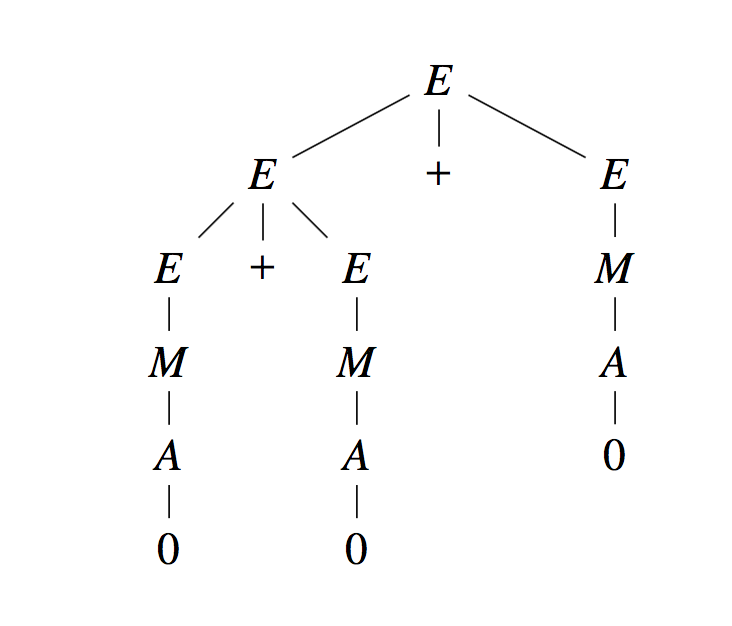
\includegraphics{syntax1}

This example generates $0+0+0$

\subsubsection{Ambiguous Grammar}

Two different trees generate the same $0+0+0$

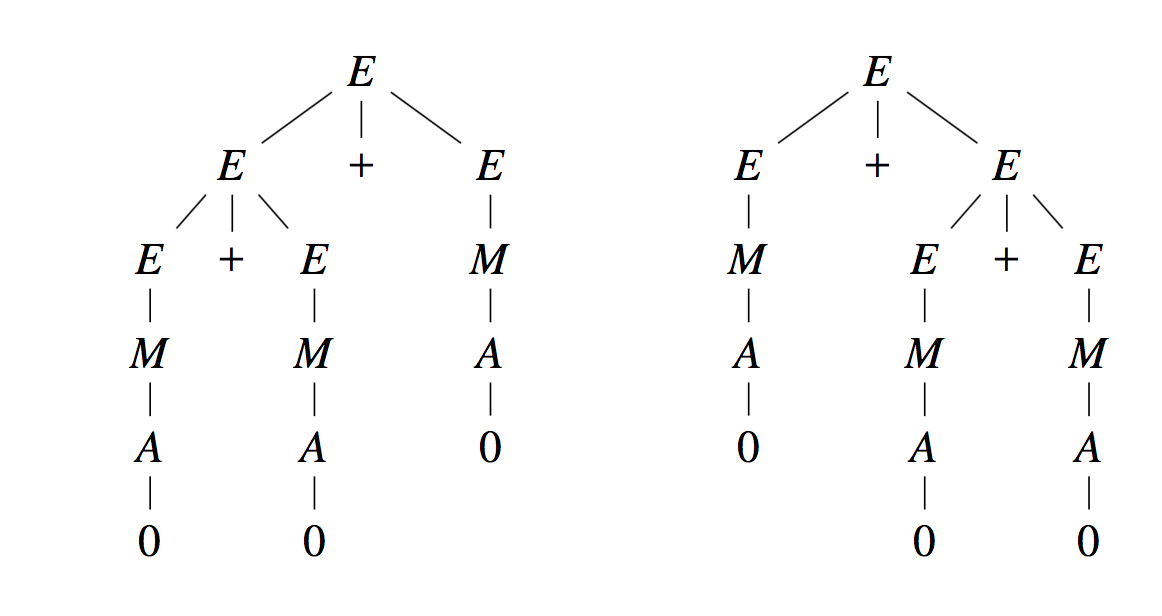
\includegraphics[scale=0.7]{syntax2}

If this happens, the grammar is ambiguous.\\
\\
We try to design unabiguous grammars.\\
\\
(Bad news: CFG ambiguity is undecidable)

\subsubsection{Ubambiguous Grammar Example}

An unambiguous grammar that generates the same language as our ambiguous grammar example:

\begin{lstlisting}
<expr> ::= <expr> "+" <expr> | <mul>
<mul> ::= <mul> "*" <mul> | <atom>
<atom> ::= "0" | "1" | "(" <expr> ")"
\end{lstlisting}

(Bad news: Equivalence of two CFGs is also undecidable)

\subsubsection{Left Recursive vs Right Recursive}

\begin{lstlisting}
<expr> ::= <expr> "+" <mul>
\end{lstlisting}
This is an example of a left recursive rule. The recursion is at the beginning (left).

\begin{lstlisting}
<expr> ::=  <mul> "+" <expr>
\end{lstlisting}
This is an example of a right recursive rule. The recursion is at the end (right).\\
\\
They affect whether infix operators associate to the left or right.\\
\\
They also affect some parsing algorithms.

\subsubsection{Recursive Descent Parsing}

Recursive descent parsing is a simple strategy for writing a parser.

\begin{itemize}
	\item{Write a procedure for each rule}
	\item{Non-terminals on Right Hand Side become procedure calls, possible recursive calls. (Thus "recursive descent". Also "top-down".) (Left-recursive grammars need special treatment.)}
	\item{Terminal symbols: Consume input and check}
	\item{Alternatives require lookahead and\slash or backtracking}
\end{itemize}

\subsubsection{Recursive Descent Parser Example}

Example grammar suitable for recursive descent parsing:

\begin{lstlisting}
<sub> ::= <atom> "-" <sub> | <atom>
<atom> ::= "0" | "1" | "(" <sub> ")"
\end{lstlisting}

Pseudo-code of recursive descent parser:

\begin{lstlisting}
sub:
	try (atom
		read; if not "-" then fail
		sub)
	if that failed: atom

atom:
	read;
	if "1" or "0": return
	if "(" : sub
		read; if not ")" then fail
	else: fail
\end{lstlisting}

\section{Thursday, March 8, 2018}

The lectures after this, Albert no longer provides lecture slides, but instead, decides to do everything in haskell files, so I will just be posting the lecture slides here and an explanation.

\subsection{ParserLib.hs}

Albert provided this really long document called "Pearl.pdf" that explained the concept of parsing, and parsers are essentially built from this one basic parser that "consumes" one character of a string and returns a result based off that input (so think of a parser consuming the $c$ of a $(c:cs)$ string, and returning some result based off that input with the rest of the unparsed string ($cs$)).

\begin{lstlisting}{language=haskell}
-- | Library of parser definition and operations.
module ParserLib where

import Control.Applicative
import Data.Char
import Data.Functor
import Data.List

newtype Parser a = PsrOf{
    -- | Function from input string to:
    --
    --   * Nothing, if failure (syntax error);
    --   * Just (unconsumed input, answer), if success.
    dePsr :: String -> Maybe (String, a)}

-- Monadic Parsing in Haskell uses [] instead of Maybe to support ambiguous
-- grammars and multiple answers.

-- | Use a parser on an input string.
runParser :: Parser a -> String -> Maybe a
runParser (PsrOf p) inp = case p inp of
                            Nothing -> Nothing
                            Just (_, a) -> Just a
                          -- OR: fmap (\(_,a) -> a) (p inp)

-- | Read a character and return. Failure if input is empty.
anyChar :: Parser Char
anyChar = PsrOf p
  where
    p "" = Nothing
    p (c:cs) = Just (cs, c)

-- | Read a character and check against the given character.
char :: Char -> Parser Char
-- char wanted = PsrOf p
--   where
--     p (c:cs) | c == wanted = Just (cs, c)
--     p _ = Nothing
char wanted = satisfy (\c -> c == wanted)   -- (== wanted)

-- | Read a character and check against the given predicate.
satisfy :: (Char -> Bool) -> Parser Char
satisfy pred = PsrOf p
  where
    p (c:cs) | pred c = Just (cs, c)
    p _ = Nothing

-- | Expect the input to be empty.
eof :: Parser ()
eof = PsrOf p
  where
    p "" = Just ("", ())
    p _ = Nothing


-- | Read and check against a given string.
string :: String -> Parser String
string wanted = PsrOf p
  where
    p inp = case stripPrefix wanted inp of
              Nothing -> Nothing
              Just suffix -> Just (suffix, wanted)
            -- Refactor this!

-- But you have to compose smaller parsers to build larger parsers and to return
-- more interesting answers, e.g., abstract syntax trees.
--
-- This is what fmap, pure, <*>, >>= are for.  And there are more...

instance Functor Parser where
    -- fmap :: (a -> b) -> Parser a -> Parser b
    fmap f (PsrOf p) = PsrOf q
                          -- (\inp -> fmap (\(rest, a) -> (rest, f a)) (p inp))
      where
        q inp = case p inp of
                  Nothing -> Nothing
                  Just (rest, a) -> Just (rest, f a)
                -- fmap (\(rest, a) -> (rest, f a)) (p inp)

instance Applicative Parser where
    -- pure :: a -> Parser a
    pure a = PsrOf (\inp -> Just (inp, a))
    -- (<*>) :: Parser (a -> b) -> Parser a -> Parser b
    -- Consider the 1st parser to be stage 1, 2nd parser stage 2.
    PsrOf p1 <*> PsrOf p2 = PsrOf q
      where
        q inp = case p1 inp of
                  Nothing -> Nothing
                  Just (middle, f) ->
                      case p2 middle of
                        Nothing -> Nothing
                        Just (rest, a) -> Just (rest, f a)
                      -- dePsr (fmap f (PsrOf p2)) middle

instance Alternative Parser where
    -- empty :: Parser a
    -- Always fail.  The identity for <|> below.
    empty = PsrOf (\_ -> Nothing)
    -- (<|>) :: Parser a -> Parser a -> Parser a
    -- Try the 1st one. If success, done; if failure, do the 2nd one
    PsrOf p1 <|> PsrOf p2 = PsrOf q
      where
        q inp = case p1 inp of
                  j@(Just _) -> j
                  Nothing -> p2 inp
    -- many :: Parser a -> Parser [a]
    -- 0 or more times, maximum munch, collect the answers into a list.
    -- Can use default implementation.

    -- some :: Parser a -> Parser [a]
    -- 1 or more times, maximum munch, collect the answers into a list.
    -- Can use default implementation.

instance Monad Parser where
    return = pure
    PsrOf p1 >>= k = PsrOf q
      where
        q inp = case p1 inp of
                  Nothing -> Nothing
                  Just (rest, a) -> dePsr (k a) rest

-- | Space or newline or tab.
whitespace :: Parser Char
whitespace = satisfy (\c -> c `elem` ['\t', '\n', ' '])

-- | Consume zero or more whitespaces, maximum munch.
whitespaces :: Parser String
whitespaces = many whitespace

-- | Read and check a terminal string, then skip trailing spaces.
terminal :: String -> Parser String
terminal wanted = string wanted <* whitespaces

-- | Read an integer, then skip trailing spaces.
integer :: Parser Integer
integer = sign <*> (read <$> some (satisfy isDigit)) <* whitespaces
  where
    sign = (char '-' *> pure negate) <|> pure id

-- | Read an identifier, then skip trailing spaces.  Disallow certain keywords.
identifier :: [String] -> Parser String
identifier keywords = do
    c <- satisfy isAlpha
    cs <- many (satisfy isAlphaNum)
    whitespaces
    let str = c:cs
    if str `elem` keywords then empty else return str

-- | One or more operands separated by an operator. Apply the operator(s) in a
-- left-associative way.
chainl1 :: Parser a               -- ^ operand parser
        -> Parser (a -> a -> a)   -- ^ operator parser
        -> Parser a               -- ^ evaluated answer
chainl1 arg op = do
    a <- arg
    more a
  where
    more x = do
        f <- op
        y <- arg
        more (f x y)
      <|>
        return x

-- | One or more operands separated by an operator. Apply the operator(s) in a
-- right-associative way.
chainr1 :: Parser a               -- ^ operand parser
        -> Parser (a -> a -> a)   -- ^ operator parser
        -> Parser a               -- ^ evaluated answer
chainr1 arg op = do
    x <- arg
    ((\f y -> f x y) <$> op <*> chainr1 arg op) <|> return x

-- | Parse a thing that is wrapped between open and close brackets.
between :: Parser open          -- ^ open bracket parser
        -> Parser close         -- ^ close bracket parser
        -> Parser a             -- ^ thing parser
        -> Parser a             -- ^ return the thing parsed
between open close p = open *> p <* close
\end{lstlisting}

\subsubsection{Parser Implementation}


So how he sets up Parsers here is that every parser returns a Maybe containing a string of the unconsumed input with $a$ being the result, and if it fails at any point, it returns Nothing. So Parsers are essentially "eating" a string, performing some functions (maybe, success or fail) and then returning the value in a way that it can be further parsed if necessary, or just Nothing if it fails along the way. It's built as a Monad so you can keep applying Parsers to a string easily, and this makes it easier to check for failure.

\subsubsection{anyChar}

the anyChar function here is a great example here, the Parser consumes one char of the string, and if eats nothing (no more string left to parse), it fails, otherwise, it succeeds and formats the output accordingly

\subsubsection{satisfy and char}

For char, it uses satisfy which uses a function that if the predicate holds true, then the Parser succeeds and returns what the Parser ate, otherwise, the Parser fails. So char specifically uses a lambda function that checks if it is the argument "wanted".

\subsubsection{eof}

This one succeeds if the Parser is called on an empty string (nothing left to eat).

\subsubsection{empty, many, and some}

Just like what the comments say, the empty Parser fails for any input, the many parser runs a parser as many times as it will succeed and populate a list with the results, and will return the list on the first failure, and the some parser does the exact same thing, but there must be at least one success, while the many parser allows for 0 successes.

\subsubsection{whitespace, terminal, integer, identifer}
whitespace just has the Parser eat one whitespace character, whitespaces eats whitepspace characters with the many parser.\\
\\
terminal eats all of the whitespaces after a string parser, and identifier eats a string and succeeds if the string is not in the list of provided strings, fails otherwise.

\subsubsection{chainl1, chainr1}
chainl1 recursively calls the "more" function if it can find more operations and arguments. It coming from the left means that it evaluates it from the left side first (so like this: $(((1+2)+3)+4)+5$).\\
\\
chainr1 does the exact same thing but on the right side this time $5+(4+(3+(1+2)))$.

\subsubsection{between}
between basically runs its open parser first, then runs the p parser, which result is returned, and then runs the close parser.

\newpage









\end{document}
